\section{Implementation}

This section discusses the implementation issues in more detail.  This chapter
concentrates on how XCPU3 was implemented and discusses implementation
decisions which have proven to be important.

\subsection{Brasil}
\emph{TODO: we need to recast this to talk about brasil as a daemon providing
the taskfs services, dynamic namespace, and serving of the local namespace --
we will mention that it is based on Inferno, but otherwise we'll tone down
the language and change the representative illustrations to match}

Inferno\cite{inferno} is an open source distributed operating system which is a 
direct descendant of the \textbf{Plan 9} operating system.  It runs natively on
multiple hardware platforms and can also run as a user-space application on
top of other operating systems.  For the purpose of this document
\textit{"hosted Inferno OS"} or \textit{"userspace Inferno"} refers to Inferno
running as user-space application on top of other operating systems.

As we are aiming for a flexible heterogeneous environment with different
operating systems and different architectures, we found the Inferno operating
system to be an attractive platform.  It allowed us to develop XCPU3 once and
easily deploy it on different platforms while enjoying the Plan 9 features
on all those platforms.

This decision does come with the cost of performance loss.  Each node needs
to run hosted Inferno in user-space which takes up some resources of the node. 
Our choice of Inferno gave us the flexibility and features of the Plan 9
operating system on other operating systems.  It allowed us to quickly
implement and deploy our filesystem on multiple platforms easily at the cost
of some performance.

XCPU3 is implemented as the filesystem in the Inferno kernel.  Figure 
\ref{fig:XCPU3} shows the placement of XCPU3 in the context of applications,
host operating system and the Inferno.

\begin{figure}[h]
  \begin{center}
    \leavevmode
      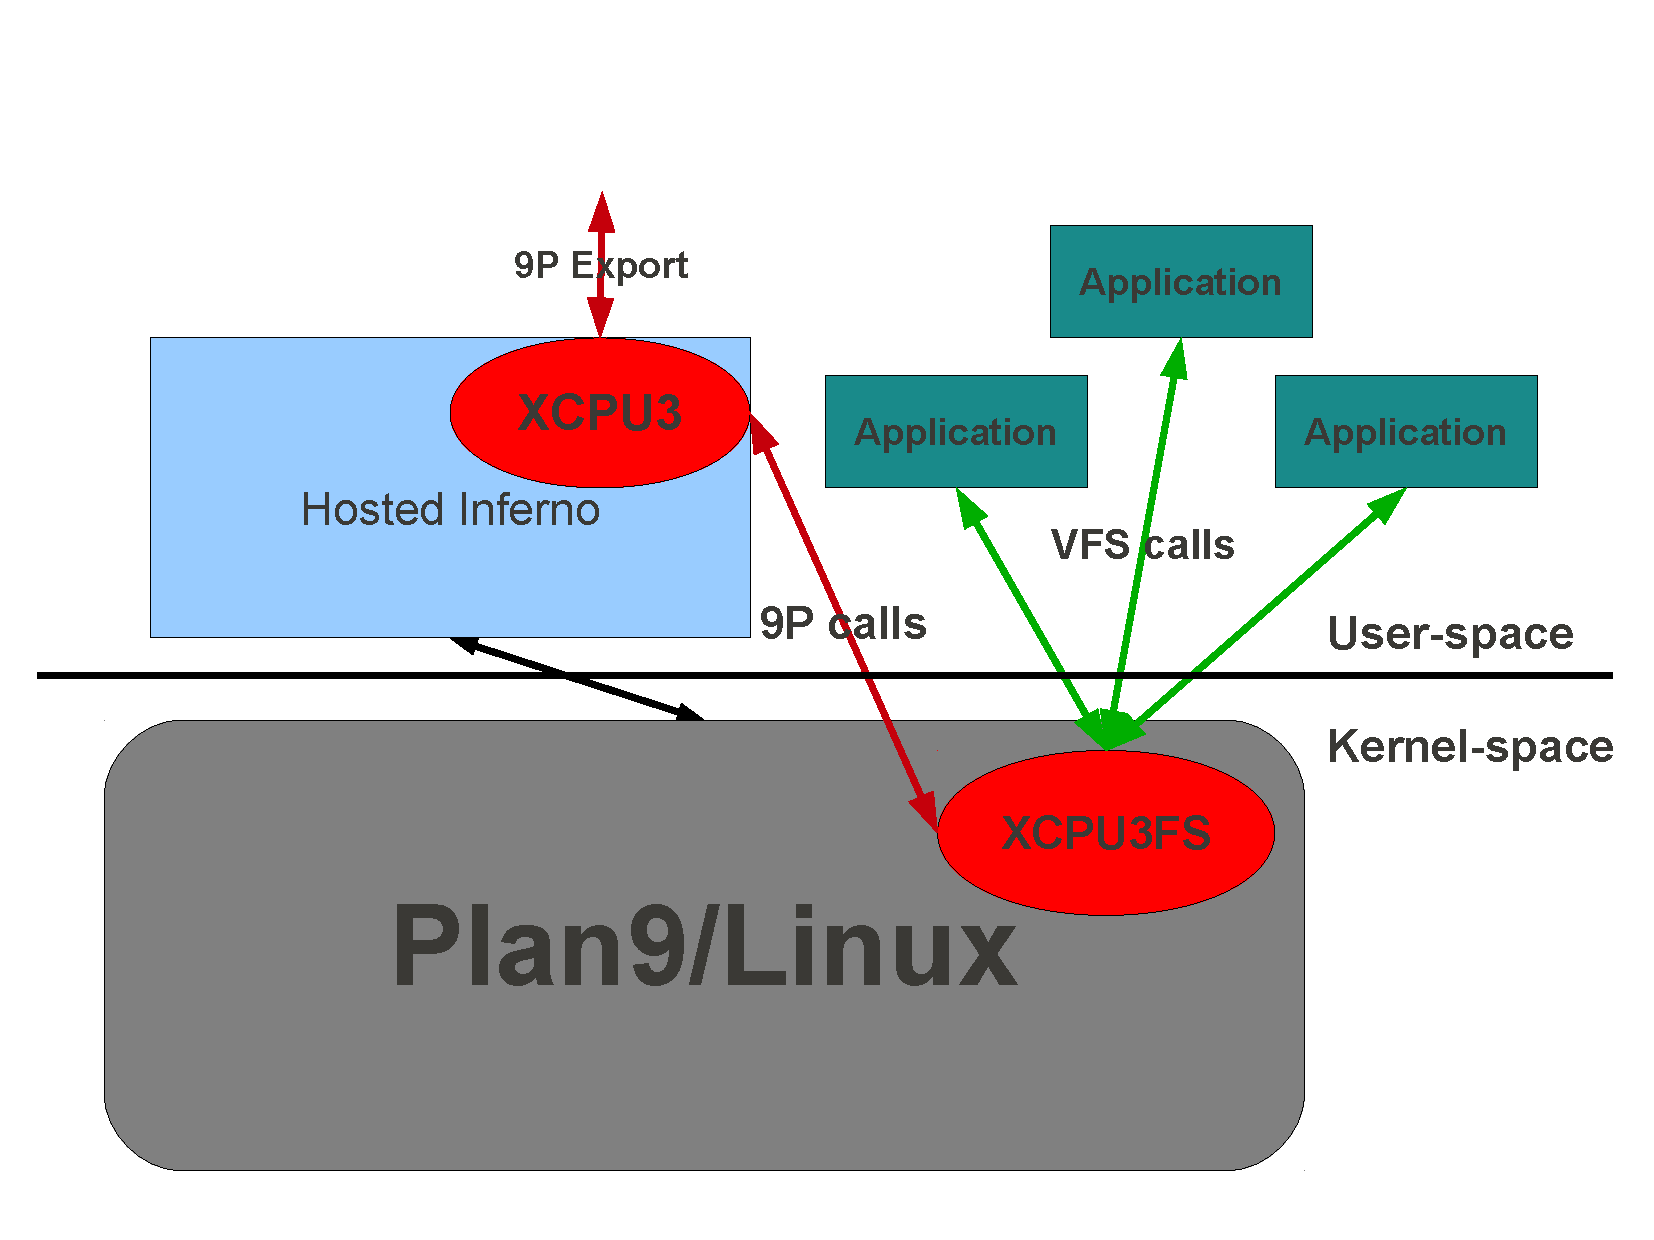
\includegraphics[height=0.2\textheight,width=0.5\textwidth]
		{./img/XCPU3Structure}
    \caption{XCPU3 Structure}
    \label{fig:XCPU3}
  \end{center}
\end{figure}

The XCPU3 filesystem is exported by Inferno using the \texttt{9P} protocol. 
This protocol is used by Plan 9 and Inferno extensively to access any file. 
Recently the Linux kernel has added support for the \texttt{9P}
protocol\cite{graverobbers}.  This allows Linux to mount filesystems
exported over the 9P protocol.  Other Unix based operating systems can use
FUSE\cite{FUSE} for accessing the 9P based filesystems. 

In a typical setup, Inferno runs in the hosted environment on an operating
system like Linux or Plan 9.  The hosted inferno will export the XCPU3
filesystem which can be mounted by the local host operating system. The 
applications interact with this mounted XCPU3 filesystem using the native
filesystem interfaces (e.g. VFS for Linux). Any interaction with this XCPU3
filesystem is communicated to Inferno using \textit{9P}. The XCPU3 kernel module
inside the inferno kernel then receives and interprets the user actions.  If
needed, it uses services from the host operating system or from other XCPU3
filesystems deployed on remote locations.  The XCPU3 filesystem then sends the
prepared response over 9P. The host operating system will relay this response
back to the application via the local filesystem interface.


\subsection{The big picture (connecting multiple XCPU3 nodes)}
The real power of the XCPU3 is the ability to connect with each other and form
bigger instance of XCPU3.  XCPU3 filesystem is exported over \texttt{9P}
providing same functionality and interface to both local and remote
applications.  This allows XCPU3 instances to connect with other XCPU3
instances and distribute some of their responsibilities among them.
The \texttt{9P} protocol shields the XCPU3 from complications of remote
filesystem access and works as transparent glue for connecting multiple XCPU3
instances together.

\subsubsection{Central Services}

The ability to configure many XCPU3 nodes into hierarchy is provided by the
\textit{central services}.  In contrary to the name, central services is
highly distributed and every XCPU3 runs an independent instance of the central
services.  


%\subsubsection{Implementation}  
The central services synthetic file server which provides a simple hierarchy of
directory mount points representing remote nodes.  Mounts of the remote nodes
or binds of previously mounted remote nodes are accomplished within this file
system such that anyone who mounts our name space can also see (and
access) anyone we have mounted transitively,  in such a way a child
node can access a parent nodes, other children, or the parents nodes
parent and so forth. Any node could establish themselves within a
hierarchy by binding a parent's central service directory to the name
\texttt{[/csrv/parent]} and then tell the parent to back-mount their name space
(allowing two way traversal).  In this way children register with parents
triggering the cross-mounts and establishing a two way link between them. Each
XCPU3 instance need to know only the information about its parent and children
in the hierarchy and the all XCPU3 nodes initiate these connections leading to
the distributed creation of the XCPU3 node hierarchy.
 
Figure \ref{fig:xcpu3FSTopo} tries to give a simple overview of how this 
synthetic filesystem view is populated based on the underlying mount
connections between the nodes.

\begin{figure}[h]
  \begin{center}
    \leavevmode
      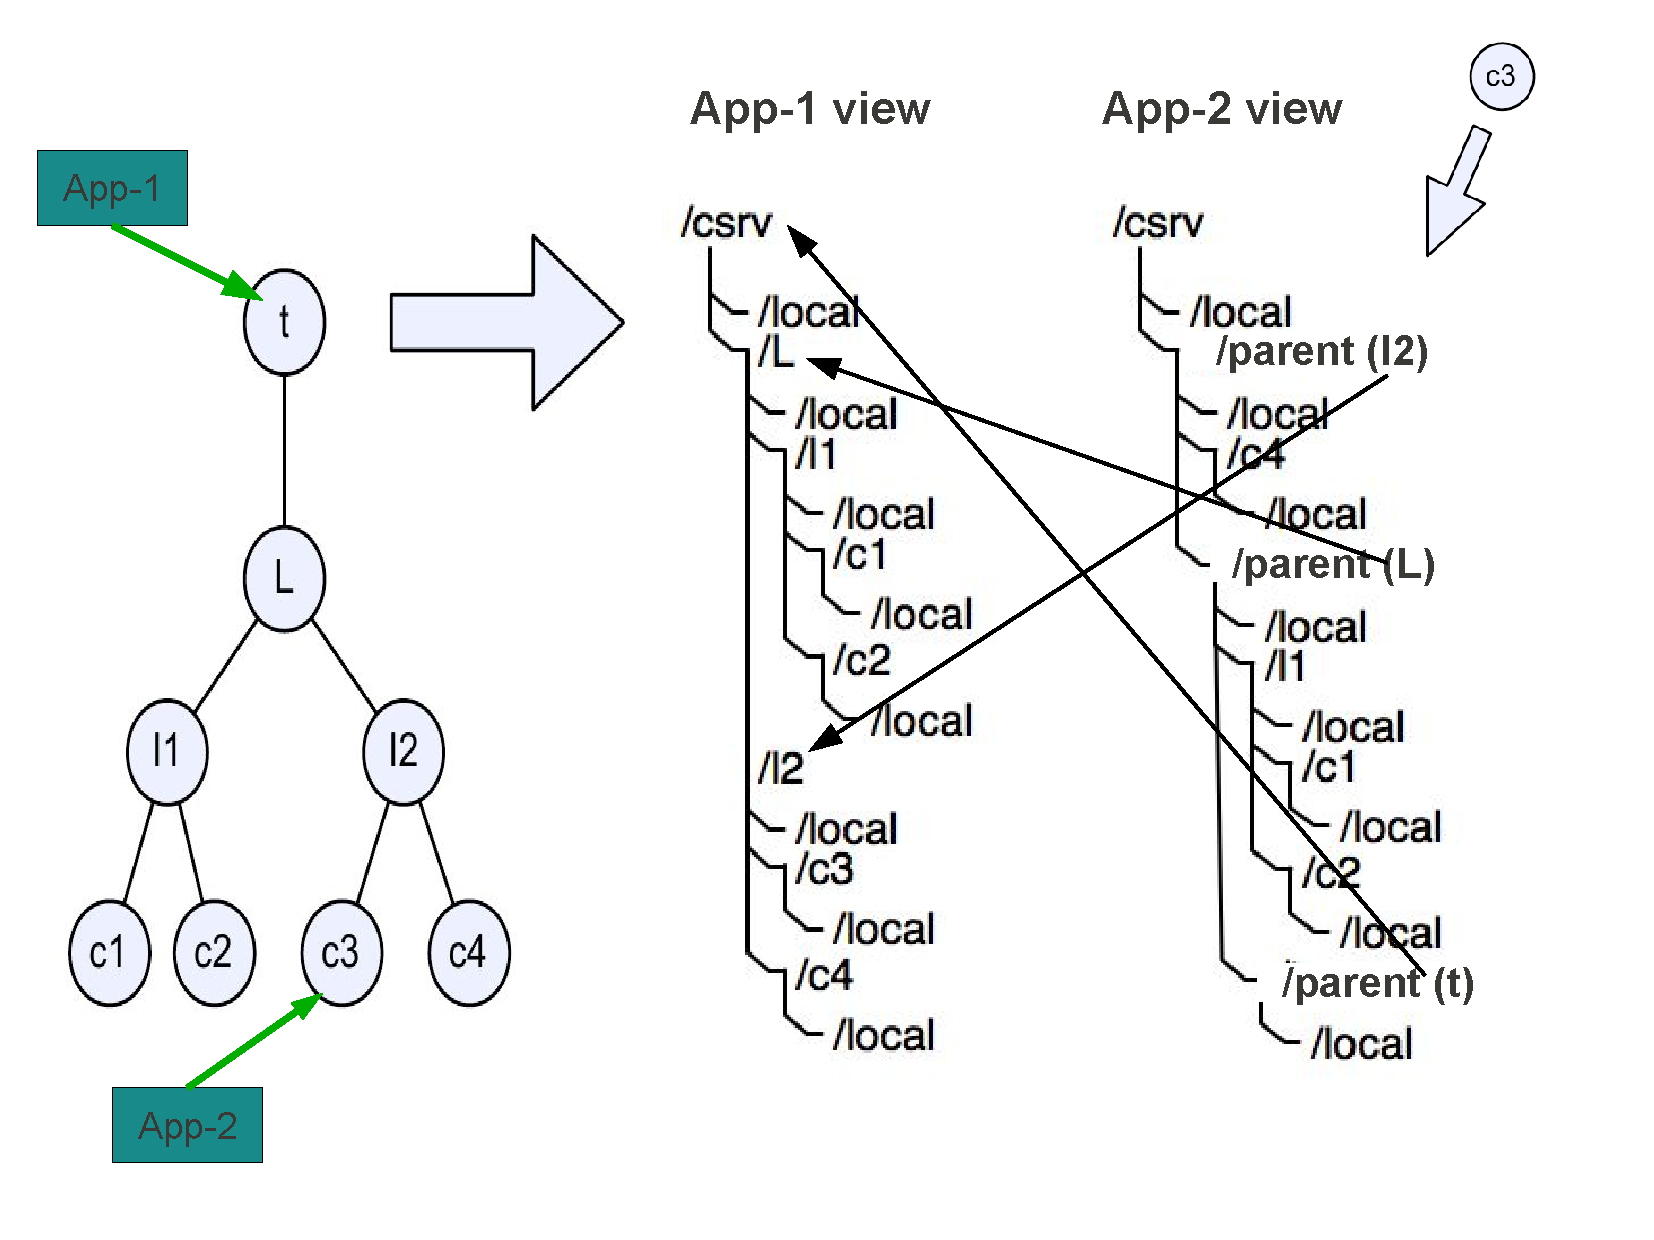
\includegraphics[height=0.3\textheight,width=0.4\textwidth]
		{./img/xcpu3FSTopo}
    \caption{Sample filesystem interface for sample the topology in XCPU3}
    \label{fig:xcpu3FSTopo}
  \end{center}
\end{figure}

Assuming the links between the nodes are created by the remote node mounts in
central services, this diagram shows how the filesystem views at different
nodes encompasses the whole network, even though each node is only connected to
its neighbours. The XCPU3 filesystem starts with the \texttt{[/csrv]}
directory. The location \texttt{[/csrv/local/]} presents the local resources
whereas \texttt{[/csrv/parent/]} presents the XCPU3 filesystem of the parent
node. All other directories in the represents the XCPU3 filesystem of the
children nodes.  It can be easily seen that both \textit{App-1} and
\textit{App-2} have access to all the nodes even though they are running on
different nodes.  In this design, every node has to worry about only its
children and the parent, other topology falls in the place automatically.

Even though the filesystem view at different nodes differ from each other, 
all nodes have access to the full topology.  The \texttt{[/csrv/]} filesystem
view encodes enough information within itself that any nodes can construct the
global view and figure out their own position within the global view.

Just because every node can construct the global view, does not mean that it
must use this global view for making any decision or performing a typical
operation. The nodes mostly use only the local view for decision making and
operations. This local view includes the parent node and the children nodes.


\section{Filesystem Interface}

This section discusses the filesystem interface and how it can be used for
managing the local and remote resources. Figure \ref{fig:xcpu3Local} gives the
the high-level view of the hierarchy of the XCPU3 filesystem.  This section
will discuss the overall hierarchy and few important files in the XCPU3.

\begin{figure}[h]
  \begin{center}
    \leavevmode
      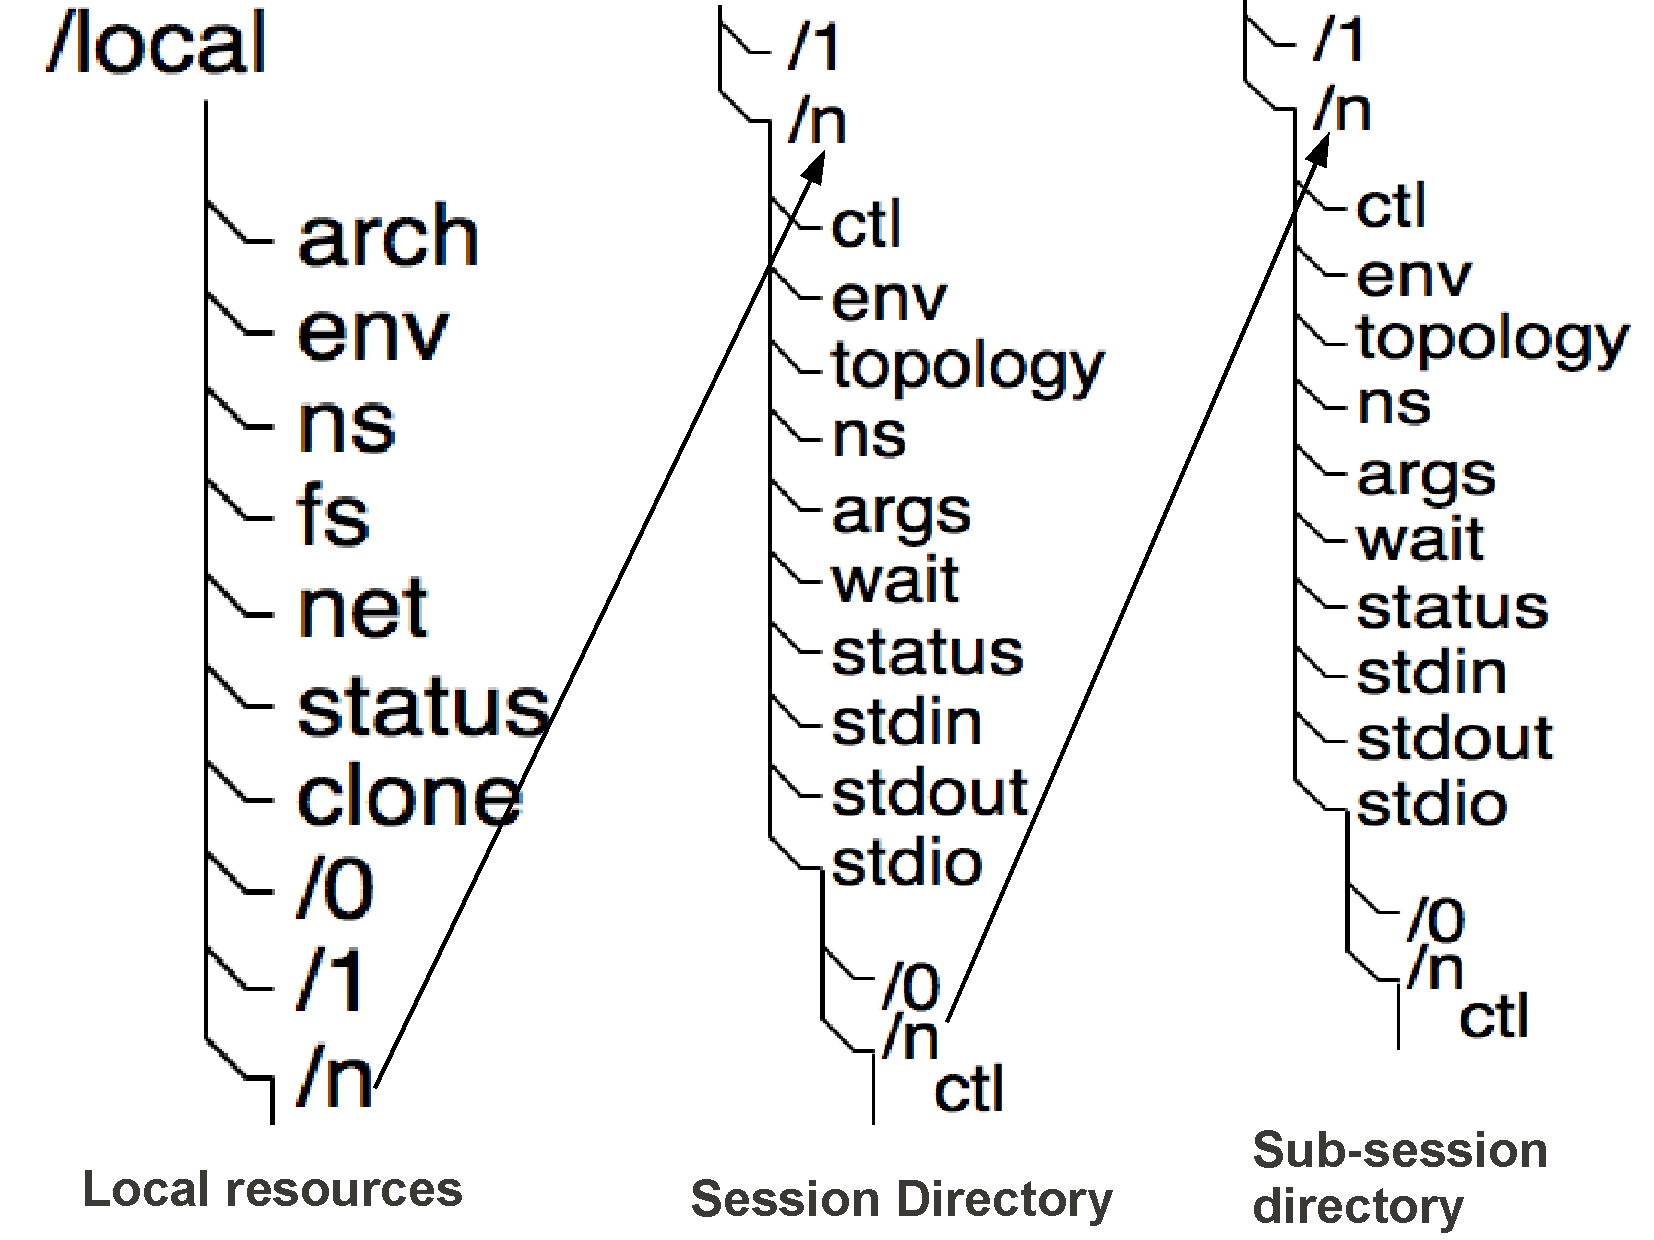
\includegraphics[height=0.25\textheight,width=0.4\textwidth]
		{./img/local_session_subsessions}
    \caption{Filesystem interface in XCPU3}
    \label{fig:xcpu3Local}
  \end{center}
\end{figure}

The location \texttt{[/csrv/local/]} points to the local resources available on
the node and the files present in this directory allows managing these local
resource. Few files here provide information about the system, like
\texttt{[arch]} file tells the architecture and operating system of the node
while \texttt{[status]} file provides information about total amount of
resources available, including the remote resources which are direct or
indirect decedents of this node.  Files like \texttt{[env]} and \texttt{[ns]}
allowed controlling the default environment and the namespace of the processes
created on this node.  \texttt{[fs]} and \texttt{[net]} are links to the local
filesystem and networking resources available on the node.  The
\texttt{[clone]} file provides the interface to create new sessions which is
the unit of the execution.

The sessions are represented as directories with session-id number as a name. 
These sessions are self-contained and provide interfaces to manage the
execution of the session.  Files like \texttt{[env]} and \texttt{[ns]} are
present is session directory also, and can be used to overwrite the default
environment and namespace specifically for this session.  File \texttt{[ctl]} is
used for controlling the execution and file \texttt{[stdio]} is used to
manipulate standard input and output.  Sessions can play one of the two roles
between \textit{single execution unit} and \textit{aggregation} of other
sessions. Following is the attempt to define these two modes.
\begin{verbatim}
SESSION -> AGGREGATION | execution
AGGREGATION -> SESSION+
\end{verbatim}
The \textbf{execution mode} executes the requested program and provides the
output.  The \textbf{aggregation} mode aggregates and manages the multiple
sessions which are created as sub-sessions for this session.  In other words,
aggregation session creates sub-sessions, divide the work among them and
aggregate back the output.  These sub-sessions are nothing but sessions created
by using \texttt{[clone]} file on local or remote systems.  These newly created
sessions are binded as sub-directories inside the current session directory.

\subsection{Workload distribution and aggregation}
The workload distribution and aggregation works by using the dual nature of
the sessions.  The first step in this is reservation, which is responsible for
creating the tree of the sessions.  Whenever any session receives the reservation
request, it evaluates it by considering, if it can execute locally or it should
break it and divide between its available children.  Depending on the decision,
it can play one of the following two roles.
\begin{enumerate}
  \item \textbf{Execution session}: When reservation is request is small enough
  or there are no children nodes available, then session behave as execution
  session by performing the requested operations locally.  The execution
  sessions are the leaf node in the session tree.
  
  \item \textbf{Aggregation session}: When request is bigger than what session
  can handle, it divides the request between children nodes.  The session does
  this by creating new session and sending the divided
  reservation request to the each child node available in it's \textbf{CSRV}
  hierarchy.  These newly created sessions will be binded as directories in the
  directory of the current session hence making them the sub-sessions of the
  current session.  The current session now acts as in aggregation point for
  these sub-sessions by passing the any execution request or input to all
  sub-sessions and merging the output from all sub-sessions to produce the final
  output.  These aggregation sessions constitute the non-leaf nodes in the
  session tree.
\end{enumerate}
This way, recursive tree of sessions is created whenever new reservation request
is received.  This tree of the session is then used to request the execution and
collect back the results.  This design not only distributes the actual
execution, but also it distributes the distribution and aggregation process as
this work is divided between all aggregation sessions.

\subsection{Examples}
It is hard to measure the \textit{ease of use} and \textit{simplicity}
factor.  So, we are presenting following examples to show how easy it is
to use XCPU3 infrastructure.  We are giving these examples of using the bash
shell in Linux.

\subsubsection{Traditional application deployment}
This example presents how the default aggregation behaviour of the XCPU3 can
used to deploy large number of applications.

We assume that the XCPU3 filesystem is mounted on \texttt{./mpoint/} directory. 
This can be done by using FUSE or 9VFS\cite{v9fseric}.
\begin{verbatim}
$ less ./mpoint/csrv/local/clone
0 
\end{verbatim}
The above command is an example of creating a new session. The contents read
from the \texttt{[clone]} file represent the session-ID.  Now we use session 0
for performing actual execution.
\begin{verbatim}
$ echo "res 4" > ./mpoint/csrv/local/0/ctl
$ echo "exec date" > ./mpoint/csrv/local/0/ctl
$ cat > ./mpoint/csrv/local/0/stdio
Fri May 7 13:53:58 CDT 2010
Fri May 7 13:53:58 CDT 2010
Fri May 7 13:53:58 CDT 2010
Fri May 7 13:53:58 CDT 2010
$
\end{verbatim}
The first echo command sends the request for reserving 4 remote resources. The
next echo command submits the request for executing the \texttt{date} command.
And the \texttt{cat} command on \texttt{[stdio]} returns the aggregated output
to the user.  This example shows all the complexities about finding, connecting
and using the remote resources is hidden behind the filesystem interface.
This approach can be used in the \textit{trivially parallelizable applications}
where the same application is deployed on all the nodes.

\subsubsection{Dataflow deployment}
In this mode the role of XCPU3 is limited to the reservation. An application
is given the capability of doing the workload distribution and aggregation
with the help of the filesystem interfaces provided by the XCPU3. Instead of
interacting with the aggregation points, these dataflow applications can
interact directly with the sessions responsible for the actual execution using
the filesystem hierarchy of that session.

In this example, we will try to create a small pipeline of two commands
\texttt{date | wc}.  But we will create this pipeline across multiple nodes. 
The objective of this example is to show how the underlying complexities are
hidden from the application.

Lets assume that session 0 is created by opening \texttt{[clone]} file as shown
in the previous example.  The following commands will create the desired
pipeline.

\begin{verbatim}
$ echo "res 2" > ./mpoint/csrv/local/0/ctl
$ echo "exec date" > ./mpoint/csrv/local/0/0/ctl
$ echo "exec wc" > ./mpoint/csrv/local/0/1/ctl
$ echo "xsplice 0 1" > ./mpoint/csrv/local/0/ctl
$ cat ./mpoint/csrv/local/0/1/stdio
1 6 29
$
\end{verbatim}

The first command \texttt{[exec date]} is sent to 0'th sub-session and the
second command \texttt{[exec wc]} is sent to the 1st sub-session.  The
\texttt{[xsplice 0 1]} request tells the parent session to redirect the output
of the 0'th session to the input of the 1st session.  The \textbf{xsplice}
command can be seen as a pipe operator of the shell script for redirecting the
output of one command to the input of other command.

The above example is equivalent of executing \texttt{date | wc} on the shell,
but with the difference that both commands are executed on a different remote
machines while sharing the same namespace.

The XCPU3 infrastructure relies on userspace applications like the \textbf{PUSH
shell}\cite{PODC:Push} for creating more complicated DAG and mapping them on
underlying XCPU3 infrastructure.
